%
% ---------------------------------------------------
%
% Trabajo Fin de Grado:
% Author: Víctor Hernández Pérez 
% Correo: alu0100697032@ull.edu.es
% Capítulo: Herramientas Software
%
% ----------------------------------------------------
%

\cleardoublepage
\chapter{Herramientas y Tecnologías Software} \label{chap:polytopes}  

En este capítulo se describen las herramientas y tecnologías que han sido usadas para la 
elaboración del trabajo, tanto la aplicación móvil como la memoria.

\section{Herramientas}
En esta sección se explicarán las herramientas de trabajo utilizadas.
\subsection{Android Studio}

Android Studio \cite{URL::AndroidStudio} es un nuevo entorno de desarrollo 
integrado para el sistema operativo Android comercializado por Google, 
diseñado para ofrecer nuevas herramientas para el desarrollo de aplicaciones y 
alternativa al entorno Eclipse \cite{URL::Eclipse}, 
hasta ahora el IDE más utilizado.
\newpage
¿Qué ofrece Android Studio? 
\begin{itemize}
\item Un entorno de desarrollo claro y robusto.
\item Facilidad para testear el funcionamiento en diversos tipos de dispositivos.
\item Asistentes y plantillas para los elementos comunes de programación en 
Android.
\item Un completo editor con muchas herramientas extra para agilizar el desarrollo 
de nuestras aplicaciones.
\end{itemize}

\begin{figure}[h]
	\centering
	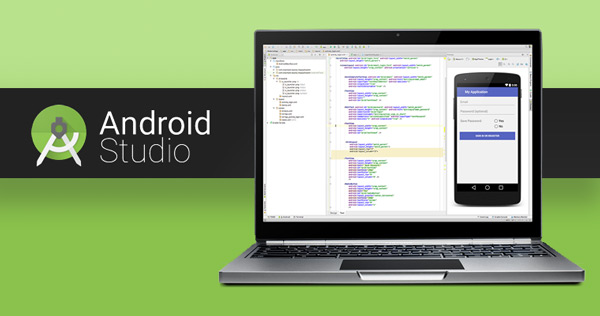
\includegraphics[width=0.7\columnwidth]{androidStudio.jpg}
	\caption{Android Studio}
	\label{fig:ejemplo}
\end{figure}

Para instalar Android Studio es necesario disponer del Java Development Kit 
(JDK) \cite{URL::JDKInfo}. 

Una vez completada la instalación del JDK, se procede a la descarga del 
AndroidStudio \cite{URL::AndroidStudio}, del SDK de Android
\cite{URL::InstallSDK} y de todos los paquetes del SDK \cite{URL::SDKPackages} 
necesarios para asegurar la compatibilidad con los dispositivos Android en
los que se desee desarrollar.
\newpage
\subsection{Atom}
\textit{Atom} \cite{URL::Atom} es un editor de texto moderno desarrollado por Github para los sistemas operativos Windows, Linux y OS X. Soporta control de versiones y 
se puede personalizar añadiendo multitud de plug-ins escritos en Node.js

\begin{figure}[h]
	\centering
	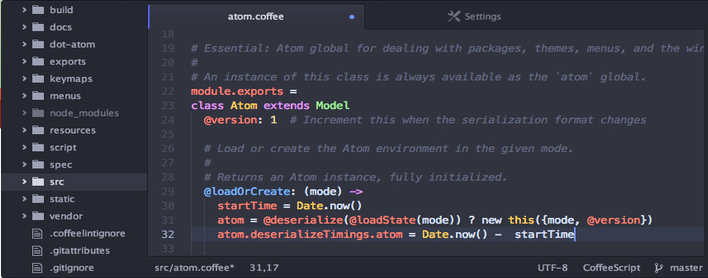
\includegraphics[width=1.0\columnwidth]{atom.png}
	\caption{Atom}
	\label{fig:ejemplo}
\end{figure}

\subsection{LaTeX y ShareLaTeX}

\textit{LaTeX} \cite{URL::LaTeX} es un sistema de composición de textos, orientado a la creación de documentos escritos que presenten una alta calidad tipográfica. 
Por sus características y posibilidades, es usado de forma especialmente intensa en la generación de artículos y libros científicos que incluyen, 
entre otros elementos, expresiones matemáticas.

\textit{ShareLaTeX} \cite{URL::ShareLatex} es un editor de LaTeX online colaborativo en tiempo real y de código libre. Y cuenta tanto con versión web como con versión de escritorio.
\newpage
\begin{figure}[h]
	\centering
	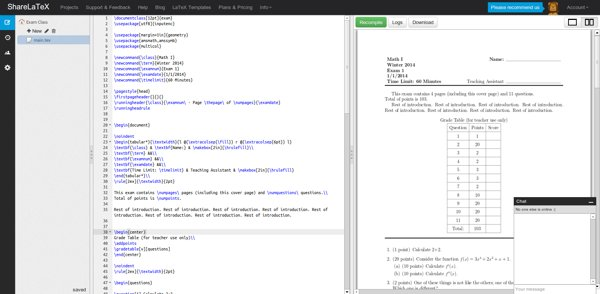
\includegraphics[width=1.0\columnwidth]{sharelatex.jpg}
	\caption{ShareLaTeX}
	\label{fig:ejemplo}
\end{figure}
\subsection{Github}
\textit{Github} \cite{URL::Github} es una plataforma de desarrollo colaborativo que sirve como repositorio de proyectos. 
Github trabaja con el sistema de control de versiones git y el código de los realizadas es almacenado 
de manera pública anunque existe también la manera de hacerlo de forma privada. 

Entre las características de esta herramienta podemos destacar:
\begin{itemize}
\item Posibilidad de tener una wiki para cada proyecto.
\item Posibilidad de tener una página web para cada proyecto.
\item Estadísticas en relación a los commits de los desarrolladores. Frecuencia, contribución y 
presentación visual de las distintas ramas del proyecto
\end{itemize}
Además la herramienta se asemeja a una red social dado que permite a cualquiera: seguir los cambios, valorar y 
ayudar a desarrollar en el proyecto.

\section{Tecnologías}
En esta sección se explicarán las tecnologías utilizadas.

\section{Sistema operativo Android}

\textit{Android} \cite{URL::Android} es un sistema operativo basado en el núcleo Linux. Fue diseñado principalmente para dispositivos 
móviles con pantalla táctil, como teléfonos inteligentes, tablets, relojes inteligentes, 
televisores y automóviles. Inicialmente fue desarrollado por Android Inc. hasta que en 2005 Google 
la compró.

Entre las características del sistema operativo se encuentran:

\begin{itemize}
\item Sevicio de mensajería, Bluetoot, videollamada etc.
\item Navegador web.
\item Multitarea.
\item Soporte para cámaras de fotos, de vídeo, pantallas táctiles, GPS, acelerómetros, 
giroscopios, magnetómetros, sensores de proximidad y de presión, sensores de luz, gamepad, 
termómetro, aceleración por GPU 2D y 3D.
\item Incluye un emulador de dispositivos, herramientas para depuración de memoria y análisis del rendimiento del software.
\item Soporte nativo para pantallas capacitivas con soporte multi-táctil.
\item Búsqueda por Google mediante voz.
\item Soporta tethering, que permite al teléfono ser usado como un punto de acceso alámbrico o inalámbrico.
\end{itemize}

\section{Django}

\textit{Django} \cite{URL::Django} es un framework web de código abierto escrito en \textit{Python} \cite{URL::Python} que sigue el patrón Modelo-Vista-Controlador. 
\newline

La meta fundamental de Django es facilitar la creación de sitios web complejos. 
Django pone énfasis en el re-uso, la conectividad y extensibilidad de componentes, el desarrollo rápido y 
el principio 'No te repitas' (DRY, del inglés Don't Repeat Yourself). Python es usado en todas las partes del 
framework, incluso en configuraciones, archivos, y en los modelos de datos.
\newline

Django necesita Python 2.5 o superior. Tiene soporte para bases de datos (PostgreSQL, MySQL y SQLite 3) y soporte de servidores web, sobretodo 
para hacer pruebas y trabajar en la etapa de desarrollo, en fase de producción se recomienda el uso de Apache.


\begin{figure}[h]
	\centering
	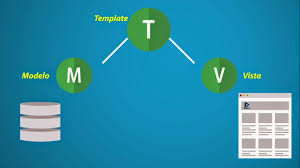
\includegraphics[width=0.5\columnwidth]{django.jpg}
	\caption{Arquitectura de Django}
	\label{fig:ejemplo}
\end{figure}

